A common problem when defining modular theory hierarchies is that the most natural include-hierarchy for the most important theories is not necessarily the same as the most comprehensive hierarchy.
For example, Ex.~\ref{syn:incl} defines \cn{Group} with an include from \cn{Monoid}.
Instead, we could include \cn{Monoid} into the intermediate theory \cn{CancellationMonoid} and include that into \cn{Group}.
This change is not possible in retrospect --- changing the theory hierarchy (which is one of the most fundamental structures of a library) usually presents an insurmountable refactoring problem.
So instead we could systematically build a hierarchy that uses every intermediate theory (as done in \cite{mathscheme}).
But this yields a very deep and complex hierarchy that is hard to navigate for casual users.
Moreover, it does not protect us from later on discovering yet another intermediate theory that should have been added.

Implicit morphisms provide a simple solution to this problem because they behave effectively like inclusions but can be added later on.
In the above example, we would
\begin{compactitem}
 \item define \cn{CancellationMonoid} with an include from \cn{Monoid},
 \item keep \cn{Group} as it is, i.e., also with an include \cn{Monoid},
 \item add an implicit morphism $\cn{CancellationMonoid}\to\cn{Group}$.
\end{compactitem}
\medskip

As a more complex example, we have built a hierarchy of theories between \cn{Band} and \cn{Semilattice}.
\ednote{@DM: this is not quite the lattice from the Wikipedia page: it consists of the 3x3 square plus Bands at the top}
All of these theories are of the form $t=\{\icl{\cn{Band}},\,a:\vdash F\}$, where $F$ is a universally quantified equational axiom.\footnote{All varieties of bands can be axiomatized in this way.}
In particular, $\cn{SemiLattice}=\{\icl{\cn{Band}},\,a:\vdash \forall [x]\forall [y] x\circ y\doteq y\circ x\}$.
Fig.~\ref{fig:bands} shows these theories.

There are various morphisms between them that describe the lattice structure of the corresponding varieties of bands.
All of these map the constants from \cn{Band} to themselves and the axiom $a$ to a proof.%
\footnote{Our formalization of the lattice of bands using implicit morphisms can be found at \url{https://gl.mathhub.info/MitM/smglom/blob/devel/source/algebra/bands.mmt}.}
We make all of these morphisms implicit.
It is straightforward to prove that the diagram commutes: any two morphisms are identical except for assignment for the axiom.
Here, \mmt can discharge the proof obligation easily using proof irrelevance.

\begin{figure}\begin{center}
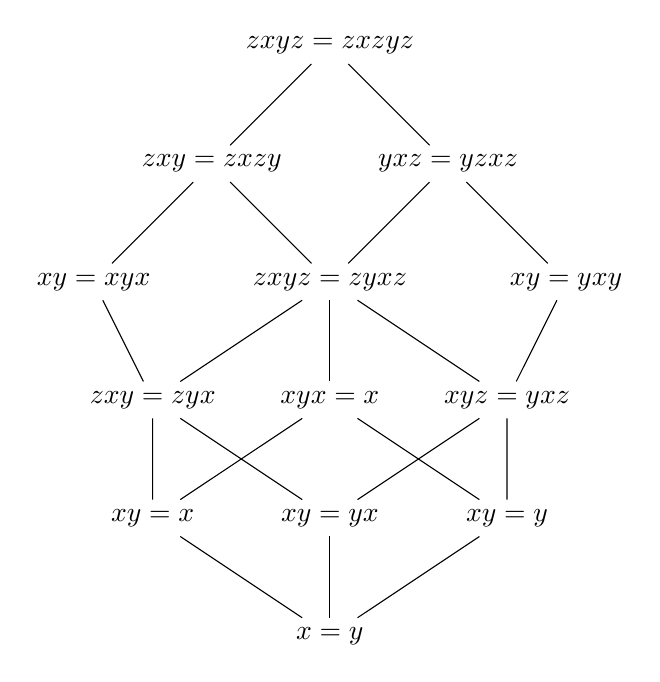
\begin{tikzpicture}[scale=1.5]
  \node (s1) at (0,0) {$zxyz=zxzyz$};
  
  \node (s2a) at (-1,-1) {$zxy=zxzy$};
  \node (s2b) at (1,-1) {$yxz=yzxz$};
  \draw (s1) to (s2a) {};
  \draw (s1) to (s2b) {};
  
  \node (s3a) at (-2,-2) {$xy=xyx$};
  \node (s3b) at (0,-2) {$zxyz=zyxz$};
  \node (s3c) at (2,-2) {$xy=yxy$};
  \draw (s2a) to (s3a) {};
  \draw (s2a) to (s3b) {};
  \draw (s2b) to (s3b) {};
  \draw (s2b) to (s3c) {};
  
  \node (s4a) at (-1.5,-3) {$zxy=zyx$};
  \node (s4b) at (0,-3) {$xyx=x$};
  \node (s4c) at (1.5,-3) {$xyz=yxz$};
  \draw (s3a) to (s4a) {};
  \draw (s3b) to (s4a) {};
  \draw (s3b) to (s4b) {};
  \draw (s3b) to (s4c) {};
  \draw (s3c) to (s4c) {};
  
  
  \node (s5a) at (-1.5,-4) {$xy=x$};
  \node (s5b) at (0,-4) {$xy=yx$};
  \node (s5c) at (1.5,-4) {$xy=y$};
  \draw (s4a) to (s5a) {};
  \draw (s4a) to (s5b) {};
  \draw (s4b) to (s5a) {};
  \draw (s4b) to (s5c) {};
  \draw (s4c) to (s5b) {};
  \draw (s4c) to (s5c) {};
  
  \node (s6) at (0,-5) {$x=y$};
  \draw (s5a) to (s6) {};
  \draw (s5b) to (s6) {};
  \draw (s5c) to (s6) {};
  
  %\node[thy,inner sep=.3cm,fill=gray] (t1) at (0,0) {};
  %\node at (t1.north west) {$S$};
  %\node at (t1) {$D$};
  %\node[thy,inner sep=.5cm,fill=lightgray] (s2) at (2,0) {};
  %\node[thy,inner sep=.3cm,fill=gray] (t2) at (2,0) {};
  %\node at (t2.north west) {$T$};
  %\node at (t2) {$C$};
  %\draw[view] (t1) to[out=10,in=170] node[above] {$\sigma$} (t2);
\end{tikzpicture}

%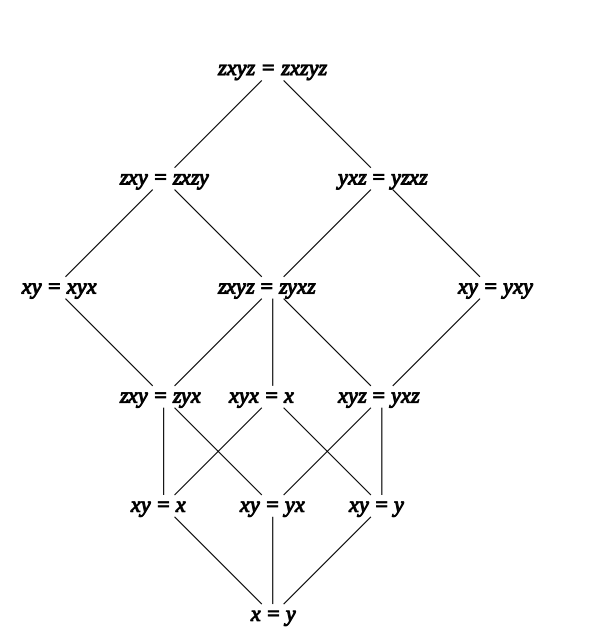
\includegraphics[width=0.6\textwidth]{bands}
\end{center}
\caption{The Lattice of Varieties of Bands}\label{fig:bands}
\end{figure}

%
%\begin{figure}
%\begin{tabular}{c|c}
%\begin{mmtcode}
%Band =
%  include ?SemiGroup
%  axiom_idemp : ⊦ ∀[x] x ∘ x ≐ x
%❚
%
%Regular =
%  include ?Band
%  axiom_regular : ⊦ ∀[x]∀[y]∀[z] 
%    z ∘ x ∘ z ∘ y ∘ z ≐ z ∘ x ∘ y ∘ z
%❚
%
%LeftNormal =
%  include ?Band
%  axiom_leftnormal : ⊦ ∀[x]∀[y]∀[z] 
%    z ∘ x ∘ z ∘ y ≐ z ∘ x ∘ y
%
%theory RightNormal =
%  include ?Band ❙
%  axiom_rightnormal : ⊦ ∀[x]∀[y]∀[z] 
%    y ∘ z ∘ x ∘ z ≐ y ∘ x ∘ z ❙ 
%❚
%
%theory Normal : ?Meta =
%  include ?Band ❙
%  axiom_normal :  ⊦ ∀[x]∀[y]∀[z] 
%    z ∘ x ∘ y ∘ z ≐ z ∘ y ∘ x ∘ z ❙
%❚
%\end{mmtcode} &
%\begin{mmtcode}
%implicit view Reg2LeftNormal : 
%    ?Regular -> ?LeftNormal =
%  include ?Band = ?Band ❙
%  axiom_regular = sketch "trivial" ❙
%❚
%
%implicit view Reg2RightNormal : 
%    ?Regular -> ?RightNormal =
%  include ?Band = ?Band ❙
%  axiom_regular = sketch "trivial" ❙
%❚
%
%implicit view LeftNormal2Normal : 
%    ?LeftNormal -> ?Normal =
%  include ?Band = ?Band ❙
%  axiom_leftnormal = sketch "trivial" ❙
%❚
%
%implicit view RightNormal2Normal : 
%    ?RightNormal -> ?Normal =
%  include ?Band = ?Band ❙
%  axiom_rightnormal = sketch "trivial" ❙
%❚
%\end{mmtcode}
%\end{tabular}
%
%\caption{Exemplary Theories for Some Varieties of Bands}\label{fig:bandsmmt}
%\end{figure}